\newpage
\section{Evaluation}
    \subsection{Determination of the threshold current}
        The current is being read out while observing the
        optical pattern on the detector card through the CCD camera.
        At a threshold current of $I_{Th}=\SI{34}{\milli\ampere}$
        the laser granulation/speckle pattern emerges,
        indicating the transition from LED-mode to lasing-mode.
        The spots visible on the detector card at a current
        immediately before and after $I_{Th}$ are shown in figure \ref{fig:Spot1} and \ref{fig:Spot2}.
        \begin{figure}[!ht]%
            \begin{subfigure}{0.46\textwidth}%
              \centering%
              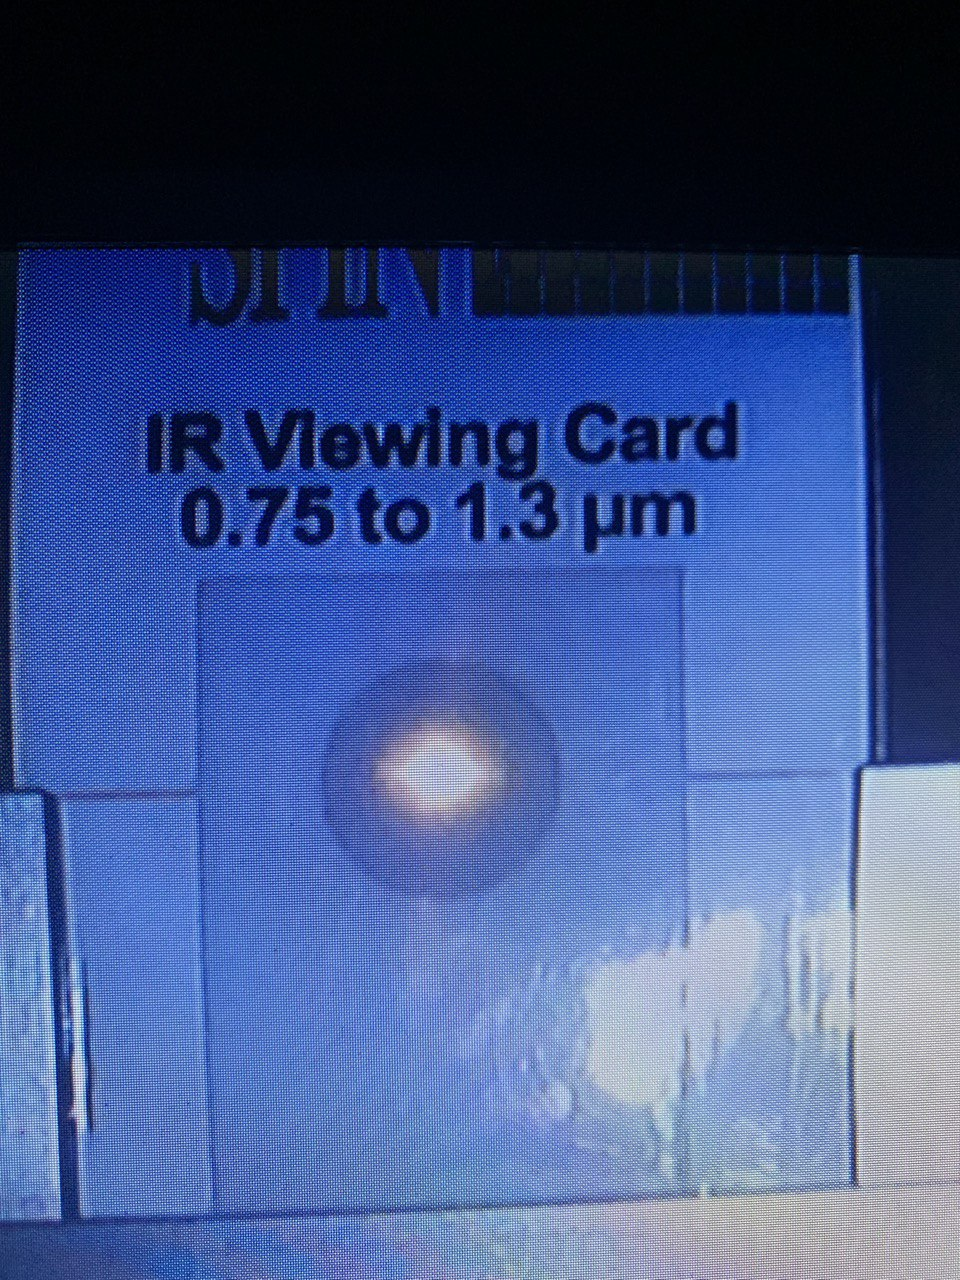
\includegraphics[scale=0.2]{pictures/Spot1.jpg}%
              \caption{Optical pattern of the diode laser in LED-mode at $I<I_{Th}$.}%
              \label{fig:Spot1}%
            \end{subfigure}%
            \hfill% Fills available space in the center -> space between figures
            \begin{subfigure}{0.46\textwidth}%
              \centering%
              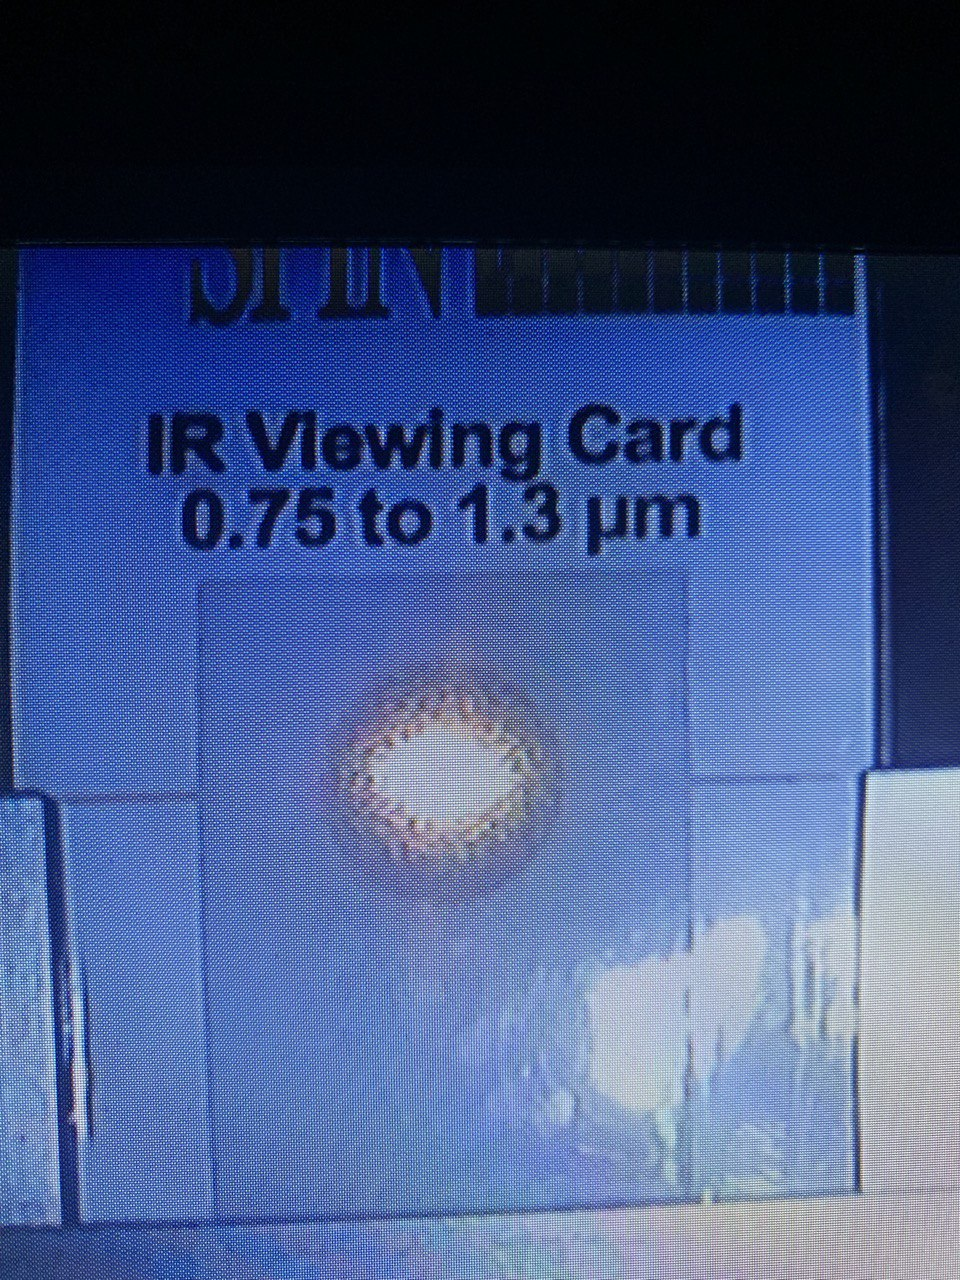
\includegraphics[scale=0.2]{pictures/Spot2.jpg}%
              \caption{Optical pattern of the diode laser in lasing-mode at $I>I_{Th}$.}%
              \label{fig:Spot2}%
            \end{subfigure}%
            \caption{Light emission on an IR-card.}%
            \label{fig:Spots}%
          \end{figure}%        
          \FloatBarrier
    \newpage
    \subsection{Recording of the rubidium fluorescence}
        The rubidium emission line, stimulated by the diode laser
        radiating through the cell and exciting the rubidium gas, is presented in figure \ref{fig:Flu}.
        \begin{figure}[h]
            \centering
            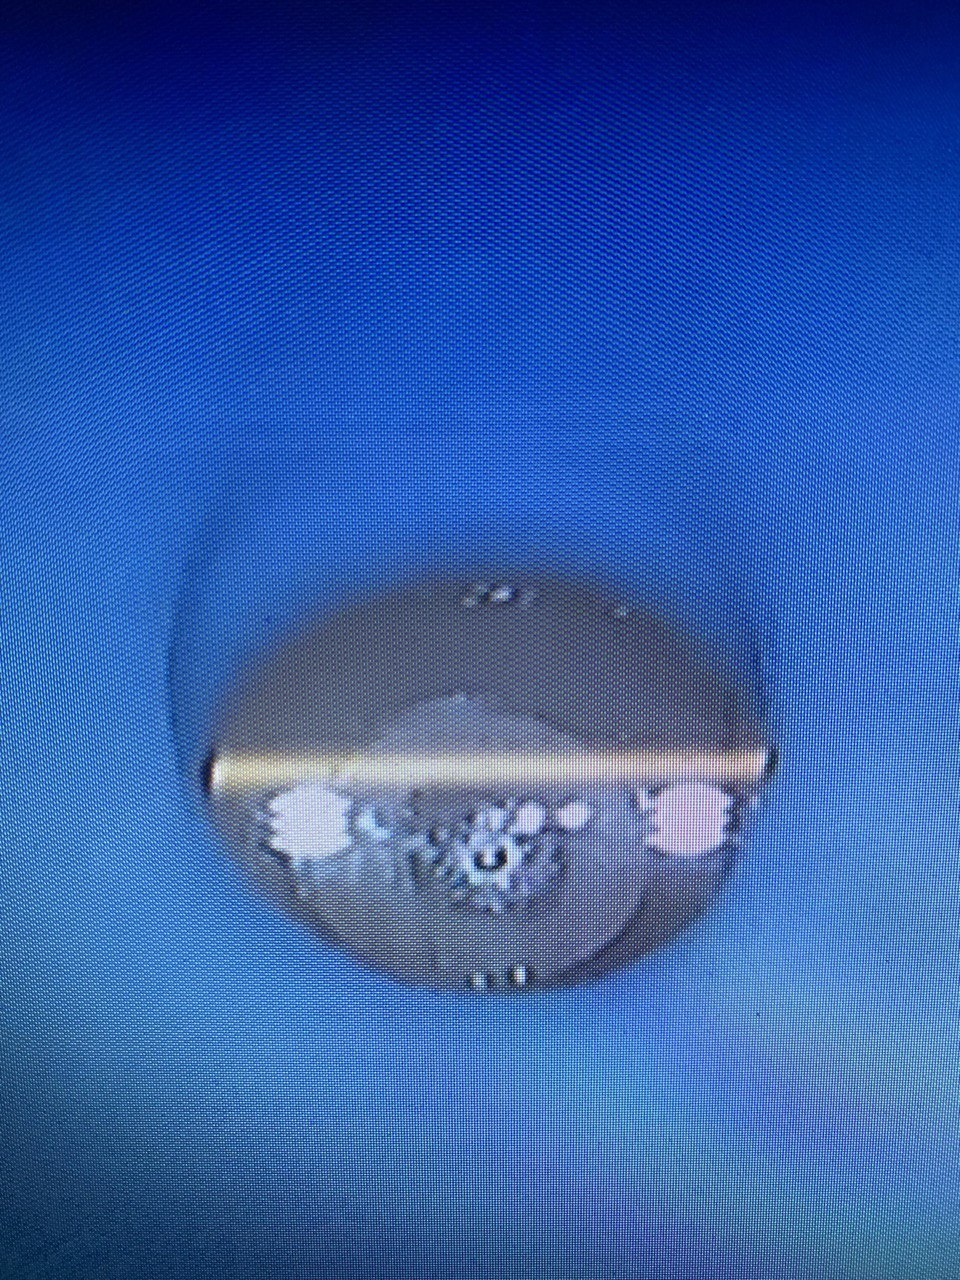
\includegraphics[width = 0.55\textwidth]{pictures/Flu.jpg}
            \caption{Rubidium fluorescence induced by the diode laser reaching the necessary photon energy.}
            \label{fig:Flu}
        \end{figure}
        \FloatBarrier
    \newpage
    \subsection{Measuring the absorption spectrum of rubidium}
        Figure \ref{fig:ES} shows the absorption spectrum of rubidium
        without any mode-hops in between the individual peaks.
        From left to right the peaks can be assigned to the
        \textit{87a}, \textit{85a}, \textit{85b} and \textit{87b}
        optical transitions of rubidium (compare with figure \ref{fig:Rb}).
        \begin{figure}[h]
            \centering
            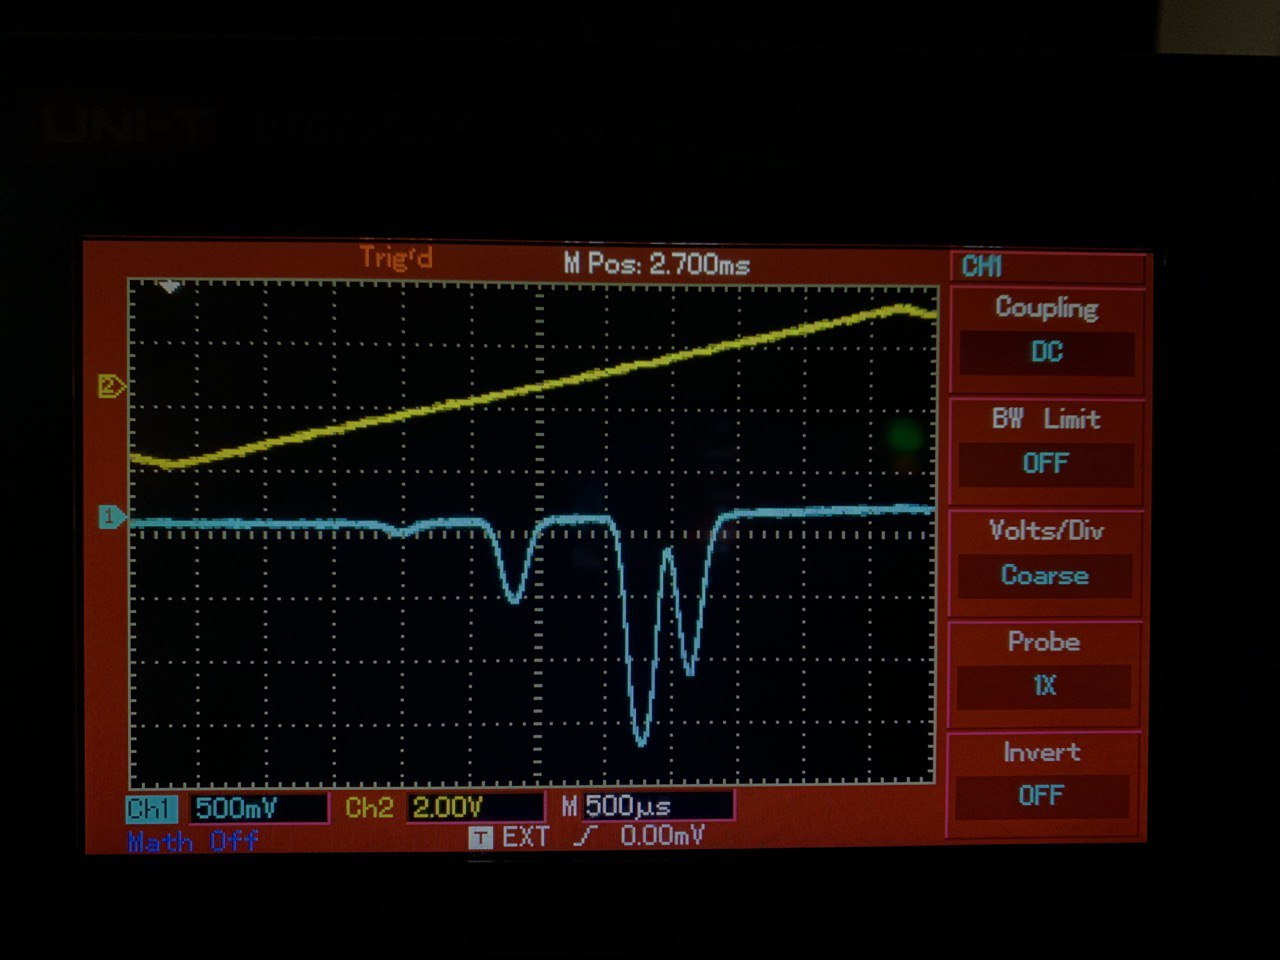
\includegraphics[width = 0.7\textwidth]{pictures/Emissionsspektrum.jpg}
            \caption{Transmission spectrum of rubidium (red).
                        The piezo-sweep is highlighted as well (blue).}
            \label{fig:ES}
        \end{figure}
